% =====================================================================
% evaluacion.tex
% Responsabilidad única: presentar la evaluación única en prueba de los
% modelos congelados, lado a lado con validación (regresión, clasificación
% y Bayes), con el umbral retrospectivo marcado como no usado.
% Cifras: macros Fin*; tablas tabla_final_*; figuras 07_*.
% =====================================================================
\section{Evaluación final en prueba}
\label{sec:evaluacion}

Antes de abrir la prueba (\FinPruebaDesde{} a \FinPruebaHasta{}) quedaron
registrados los modelos congelados (Tabla~\ref{tab:congelado}), y la prueba
se leyó una sola vez, en la etapa~07; nada de lo que sigue se usó para cambiar
un modelo, una variable o un umbral.

\begin{table}[!htbp]
\centering
\tablaancha{final_congelado}
\caption{Modelos congelados antes de abrir la prueba, con la cifra de
validación que justificó cada uno.}
\label{tab:congelado}
\end{table}

\subsection{Regresión}

En los \FinDiasPrueba{} días hábiles de prueba, la regresión lineal obtuvo un
RMSE de \FinRMSEPrueba{} (IC 95\,\% de \FinRMSEPruebaInf{} a
\FinRMSEPruebaSup{}), un MAE de \FinMAEPrueba{}, un $R^2$ de
\FinRDosPrueba{} y una habilidad de \FinHabilidadPrueba{} (de
\FinHabilidadPruebaInf{} a \FinHabilidadPruebaSup{}) frente a
\codigo{\FinRegReferencia} (Tabla~\ref{tab:final-reg}). El RMSE cambió un
\FinCambioRMSEPct{}\,\% respecto a validación, es decir, el modelo se
equivocó menos en prueba, pero eso no prueba que haya mejorado: la carga media
de prueba (\FinMediaPrueba{} muestras por día hábil) es menor que la de
validación (\RegMediaValidacion{}), y con un nivel más bajo los errores
absolutos también tienden a serlo. La habilidad, que se mide frente a la
referencia del mismo periodo, también subió, y su intervalo se solapa con el
de validación, así que lo prudente es leer ambos periodos como compatibles.

\begin{table}[!htbp]
\centering
\small
\tablagen{final_regresion_validacion}
\caption{Regresión: validación frente a prueba, con intervalo bootstrap de
95\,\% en prueba.}
\label{tab:final-reg}
\end{table}

\begin{figure}[!htbp]
\centering
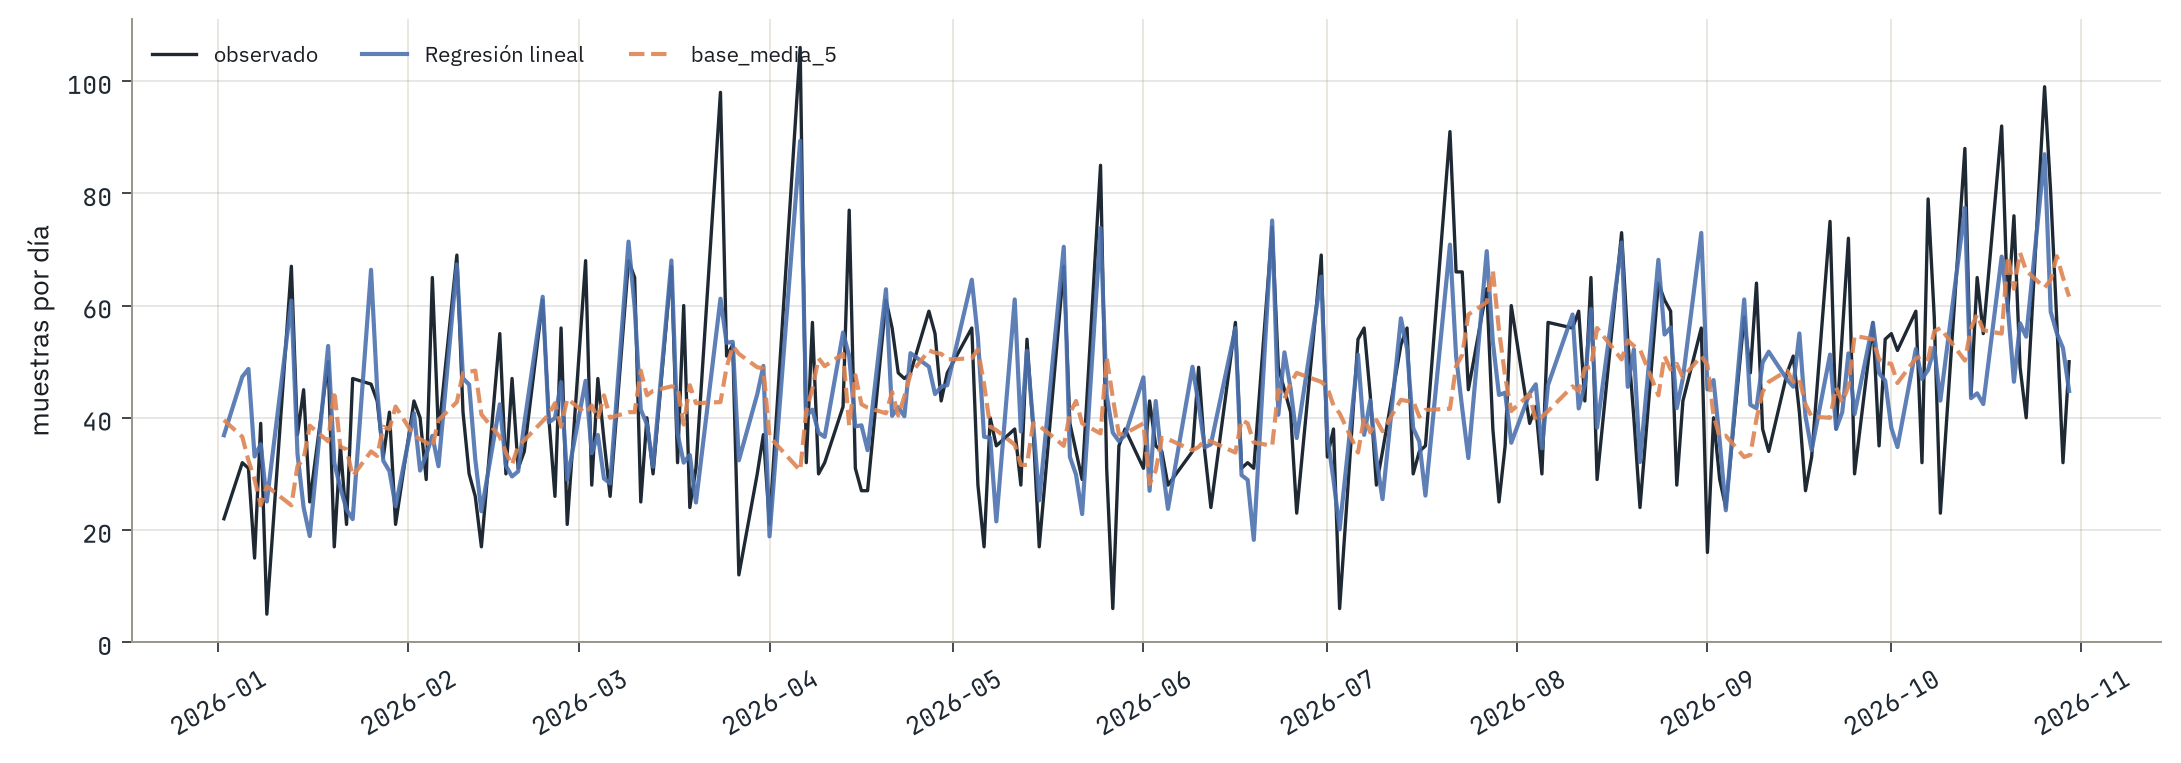
\includegraphics[width=0.85\textwidth]{07_serie_prueba.png}
\caption{Serie de prueba: observado (negro), regresión lineal congelada (azul)
y media de los cinco días anteriores (naranja). Conviene mirar los primeros
días de enero, donde el modelo sobreestima la carga, y los picos aislados, que
ningún predictor anticipa.}
\label{fig:final-serie}
\end{figure}

El error no es uniforme en el tiempo (Figura~\ref{fig:final-serie}): en los
\FinDiasFinDeAnio{} días hábiles de la ventana de fin de año, el residuo medio
es de \FinResiduoFinDeAnio{} muestras (el modelo predice de más), frente a
\FinResiduoResto{} en el resto, lo que indica que el calendario del modelo no
captura bien el arranque lento de enero. En términos operativos, el
\FinDiasFueraPct{}\,\% de los días queda fuera de la tolerancia práctica,
frente al \FinDiasFueraReferenciaPct{}\,\% de la referencia.

\subsection{Clasificación}

La regresión logística calibrada mantuvo su capacidad de ordenar, con un
ROC-AUC de \FinAUCPrueba{} (IC 95\,\% de \FinAUCPruebaInf{} a
\FinAUCPruebaSup{}) frente a \ClfAUCValidacion{} en validación, y su
calibración, con una probabilidad media de \FinProbMediaPrueba{} frente a una
tasa real de \FinPrevalenciaPrueba{} y un Brier de \FinBrierPrueba{}
(Tabla~\ref{tab:final-clf}). Con el umbral congelado ($t=\FinUmbral$) la
precisión casi no cambió (\FinPrecisionPrueba{}, de \FinPrecisionPruebaInf{}
a \FinPrecisionPruebaSup{}), pero el recall bajó de \ClfRecallUmbral{} a
\FinRecallPrueba{} (de \FinRecallPruebaInf{} a \FinRecallPruebaSup{}), con
$\text{TP}=\FinTP$, $\text{FP}=\FinFP$, $\text{FN}=\FinFN$ y
$\text{TN}=\FinTN$ en las \FinMuestrasPrueba{} muestras con resultado.

\begin{table}[!htbp]
\centering
\small
\tablagen{final_clasificacion_validacion}
\caption{Clasificación: validación frente a prueba con el umbral congelado,
con intervalo bootstrap de 95\,\% en prueba.}
\label{tab:final-clf}
\end{table}

Las alertas bajaron a \FinAlertasSemana{} por semana en las
\FinSemanasPrueba{} semanas de prueba (frente a \ClfAlertasSemana{} en
validación), en parte porque llegan menos muestras por día. El costo fue de
\FinCostoPrueba{} (\FinCostoPorMuestraPrueba{} por muestra), frente a
\FinCostoNoAlertar{} de no alertar y \FinCostoAlertarTodo{} de alertar todo,
un ahorro del \FinAhorroPct{}\,\% frente a la mejor política sin modelo, algo
menor que el \ClfAhorroPct{}\,\% de validación.

\paragraph{Umbral retrospectivo (no se usa).} Mirando la prueba, el umbral de
menor costo habría sido \FinUmbralRetro{}, con un costo de \FinCostoRetro{}
frente a \FinCostoPrueba{} del umbral congelado. Se reporta solo para medir
cuánto se pierde por decidir sin ver la prueba, una diferencia pequeña, y
\textbf{no se adopta}, porque elegirlo con la prueba invalidaría la
evaluación.

\subsection{Probabilidad de falso positivo}

En prueba, los \FinReensayados{} positivos reensayados dieron un
\FinReensayoConformeObservadoPct{}\,\% de reensayos conformes (Wilson de
\FinReensayoConformeObservadoInfPct{}\,\% a
\FinReensayoConformeObservadoSupPct{}\,\%), y la capa bayesiana, con la
sensibilidad y la especificidad del desarrollo, anticipaba un
\FinReensayoConformeEsperadoPct{}\,\%, dentro de ese intervalo. El VPP$(x)$
medio de los positivos de prueba es de \FinVPPxMedio{}, es decir, uno de cada
\FinUnoDeCadaFalso{} positivos sería falso. La regla de reensayo se sostiene: bajo el borde, el \FinReglaTasaBajoPct{}\,\% de
los reensayos fue conforme (Wilson de \FinReglaTasaBajoInfPct{}\,\% a
\FinReglaTasaBajoSupPct{}\,\%, con \FinReglaBajoBorde{} de los
\FinReglaReensayosConRecuento{} reensayos con recuento), frente al
\FinReglaTasaAltoPct{}\,\% sobre él, y el grupo concentró el
\FinReglaCapturaPct{}\,\% de los reensayos conformes.

Por ensayo, \FinEnsayosPocosPositivos{}
ensayos tienen menos de \FinMinimoPositivos{} positivos en prueba
(\textit{Salmonella} y esterilidad), así que sus fracciones observadas son
poco precisas y no se interpretan. En la auditoría con la verdad de la
simulación, la fracción de positivos de prueba realmente contaminados es de
\FinAudVPPReal{}, cercana al VPP$(x)$ medio, y el Brier del VPP$(x)$
(\FinAudBrierVPPx{}) vuelve a ser menor que el del VPP por ensayo
(\FinAudBrierVPPEnsayo{}).

\subsection{Resumen}

La Tabla~\ref{tab:final-resumen} reúne las cifras principales. Ninguna se
degradó de forma que invalide el modelo correspondiente, y entre las métricas de desempeño
la que más empeoró es el recall de la clasificación, que conviene vigilar con los datos reales. El
agrupamiento no tiene evaluación en prueba, porque es descriptivo
(\FinAgrK{} perfiles de muestra con silueta \FinAgrSilueta{} y
\FinAgrSegmentos{} segmentos de clientes).

\begin{table}[!htbp]
\centering
\small
\tablagen{final_resumen}
\caption{Resumen final: validación (o desarrollo, en Bayes) frente a prueba.}
\label{tab:final-resumen}
\end{table}
